
\begin{figure}[h!]
    \centering
    \caption{Desempenho dos modelos de regressão aplicados para inferir as leituras de concentração de \acrshort{co} medidas pela estação de referência}
    \begin{subfigure}{0.9\textwidth}
        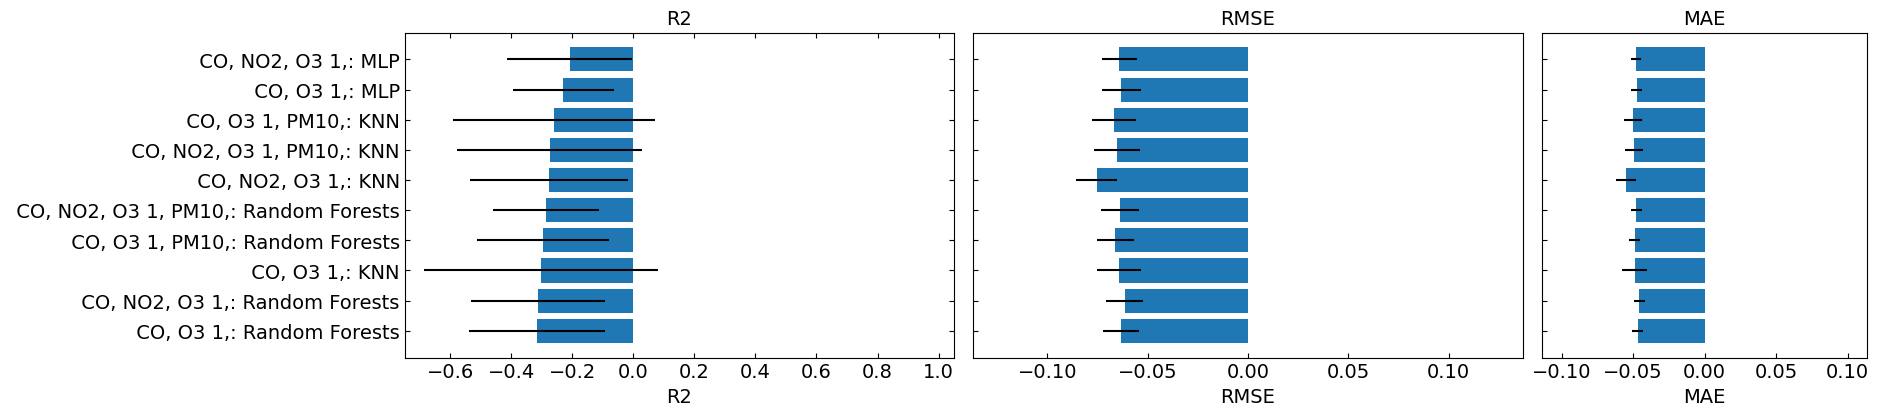
\includegraphics[width=\textwidth]{chapters/4-CALIBRAÇÃO MÚLTIPLOS SENSORES/Figuras/co-all-models-performance.png}
        \caption{Valores de R2, RMSE e MAE obtidos pelos 10 modelos com maiores valores de R2}
        \label{fig:data-co-all-models-performance}
    \end{subfigure}
    \begin{subfigure}{0.9\textwidth}
        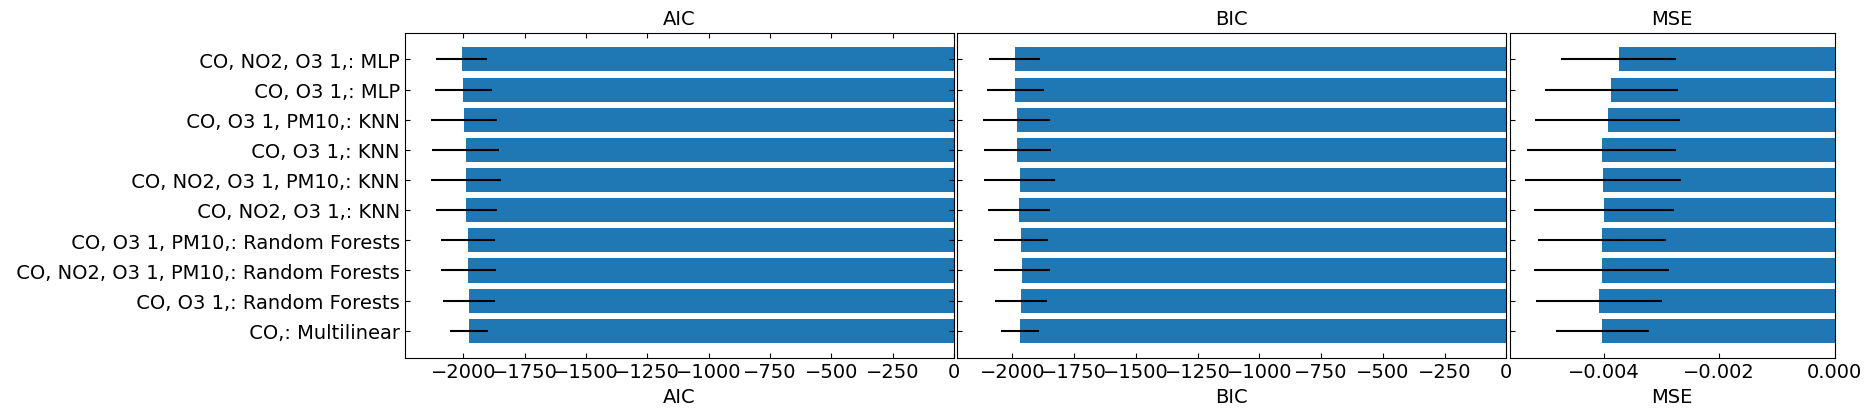
\includegraphics[width=\textwidth]{chapters/4-CALIBRAÇÃO MÚLTIPLOS SENSORES/Figuras/co-all-models-complexity.png}
        \caption{Modelos com menores valores de \acrshort{aic} e \acrshort{bic}}
        \label{fig:data-co-all-models-complexity}
    \end{subfigure}
    \label{fig:data-co-all-models-performance-comlexity}
\end{figure}

% ----------------------------------------------------------
\section{Calibração das leituras de Monóxido de Carbono}
% ----------------------------------------------------------

A Figura \ref{fig:data-co-all-models-performance} apresenta os valores de R2 dos 10 melhores modelos de calibração calculados para as leituras de \acrshort{co}. Observa-se que apesar do valor médio de R2 obtido nas validações cruzadas continuar sendo negativo, obtiveram-se máximos de até aproximadamente 0.1 para alguns conjuntos de dados de teste nas validações cruzadas. Em geral os modelos que produziram os melhores resultados foram baseados em regressões pelos k vizinhos mais próximos e redes neurais Perceptron Multicamadas. Com relação as variáveis de entrada dos modelos, todos os que produziram melhores resultados consideraram as leituras do sensor 1 de \acrshort{o3}. Outros que obtiveram valores positivos de R2 tiveram como variáveis de entrada o \acrshort{mp10} e \acrshort{no2}.

\begin{figure}[h]
    \centering
    \caption{Gráfico de dispersão das leituras do múltiplos sensores e a estação de referência para medição de \acrshort{co}}
    \begin{subfigure}{0.49\textwidth}
        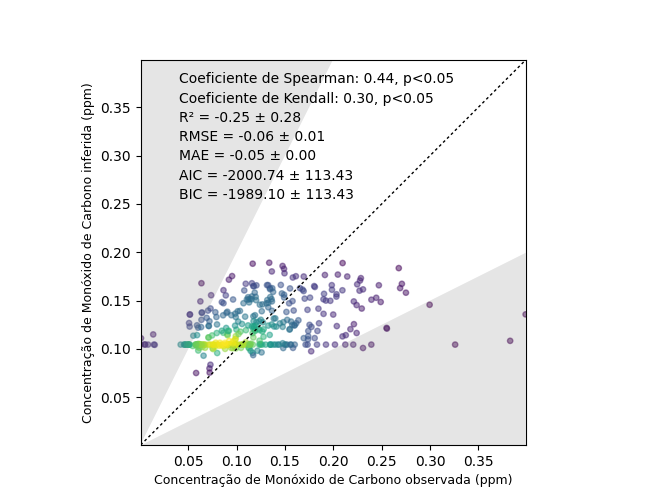
\includegraphics[width=\textwidth]{chapters/4-CALIBRAÇÃO MÚLTIPLOS SENSORES/Figuras/CO-co-o31-mlp-Regression.png}
        \caption{Utilizando modelo de regressão com uma rede neural Perceptron Multicamadas; variáveis independentes: leituras de sensores CO-B4 e OX-B431 (1)}
        \label{fig:data-co-o31-reference-corr-MLP}
    \end{subfigure}
    \hfill
    \begin{subfigure}{0.49\textwidth}
        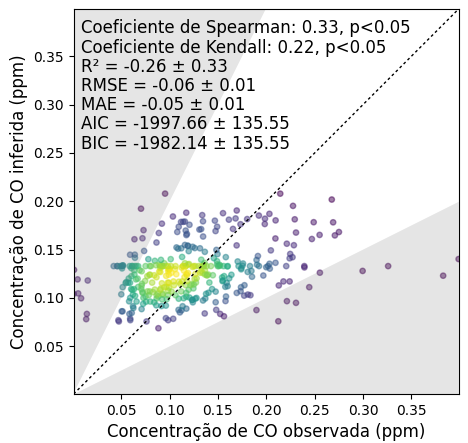
\includegraphics[width=\textwidth]{chapters/4-CALIBRAÇÃO MÚLTIPLOS SENSORES/Figuras/CO-co-o31-pm10-knn-Regression.png}
        \caption{Utilizando modelo de regressão pelos k vizinhos mais próximos; variáveis independentes: leituras de sensores CO-B4, OX-B431 (1) e de \acrshort{mp10} medido pelo OPC-N3}
        \label{fig:data-co-o31-mp10-reference-corr-KNN}
    \end{subfigure}
\end{figure}

Ao comparar os modelos em termos de sua complexidade, observa-se uma sobreposição entre os que desempenharam melhor em termos de representação dos dados originais (maiores valores de R2) e os que desempenharam melhor em termos de complexidade (menores valores de AIC e BIC). A Figura \ref{fig:data-co-all-models-complexity} compara os valores de \acrshort{aic}, \acrshort{bic} e \acrshort{mse} dos 10 modelos que obtiveram menores valores de AIC. Por último as Figuras \ref{fig:data-co-o31-reference-corr-MLP} e \ref{fig:data-co-o31-mp10-reference-corr-KNN} mostram gráficos de dispersão entre os valores de saída dos modelos de calibração e os dados de referência de \acrshort{co}. Os gráficos mostram os resultados dos modelos com melhores valores de R2.